%---------change this every homework
\def\yourid{Hyun Suk Ryoo}
\def\collabs{}
% -----------------------------------------------------
\def\duedate{9/20/18 12:30PM}
\def\duelocation{via Collab}
\def\prof{hr2ee}
\def\course{{Math 3100 (Introduction to Probability)}}%------
%-------------------------------------
%-------------------------------------

\documentclass[10pt]{report}
\usepackage[colorlinks,urlcolor=blue]{hyperref}
\usepackage[osf]{mathpazo}
\usepackage{amsmath,amsfonts,graphicx}
\usepackage{latexsym}
\usepackage[shortlabels]{enumitem}
\usepackage[top=1in,bottom=1.4in,left=1.5in,right=1.5in,centering]{geometry}
\usepackage{color}
\definecolor{mdb}{rgb}{0.3,0.02,0.02} 
\definecolor{cit}{rgb}{0.05,0.2,0.45} 
\pagestyle{myheadings}
\markboth{\yourid}{\yourid}
\usepackage{clrscode}
\usepackage{url}

\newenvironment{proof}{\par\noindent{\it Proof.}\hspace*{1em}}{$\Box$\bigskip}
\newcommand{\handout}{
   \renewcommand{\thepage}{}
   \noindent
   \begin{center}
      \vbox{
    \hbox to \columnwidth {\sc{\course} --- \prof \hfill}
    \vspace{-2mm}
    \hbox to \columnwidth {\sc due \MakeLowercase{\duedate} \duelocation \hfill {\LARGE\color{mdb}\yourid}}
      }
   \end{center}
      Homework \# 3
   \vspace*{2mm}
}
\newcommand{\solution}[1]{\medskip\noindent\textbf{Solution:}#1}
\newcommand{\bit}[1]{\{0,1\}^{ #1 }}
%\dontprintsemicolon
%\linesnumbered
\newtheorem{problem}{\sc\color{cit}section}
\newtheorem{practice}{\sc\color{cit}practice}
\newtheorem{lemma}{Lemma}
\newtheorem{definition}{Definition}

\def\therefore{\boldsymbol{\text{ }
\leavevmode
\lower0.4ex\hbox{$\cdot$}
\kern-.5em\raise0.7ex\hbox{$\cdot$}
\kern-0.6em\lower0.4ex\hbox{$\cdot$}
\thinspace\text{ }}}

\begin{document}
\thispagestyle{empty}
\handout
%----Begin your modifications here

\setcounter{chapter}{1} 
\ \\
{\color{cit}A problem on the Polya urn...} \\

Let initially a box contain 2 red and 1 blue ball. At each step we draw a random ball from the box, and add 2 balls of the same color back. What is the probability that after 3 steps there will be 4 red and 2 blue balls in the box? (note: the answer might not be uniform because we start from 2 red and 1 blue, and not like it was in class)
\begin{center}
The probability is $\frac{18}{60} \rightarrow \mathbf{0.3} $ \\
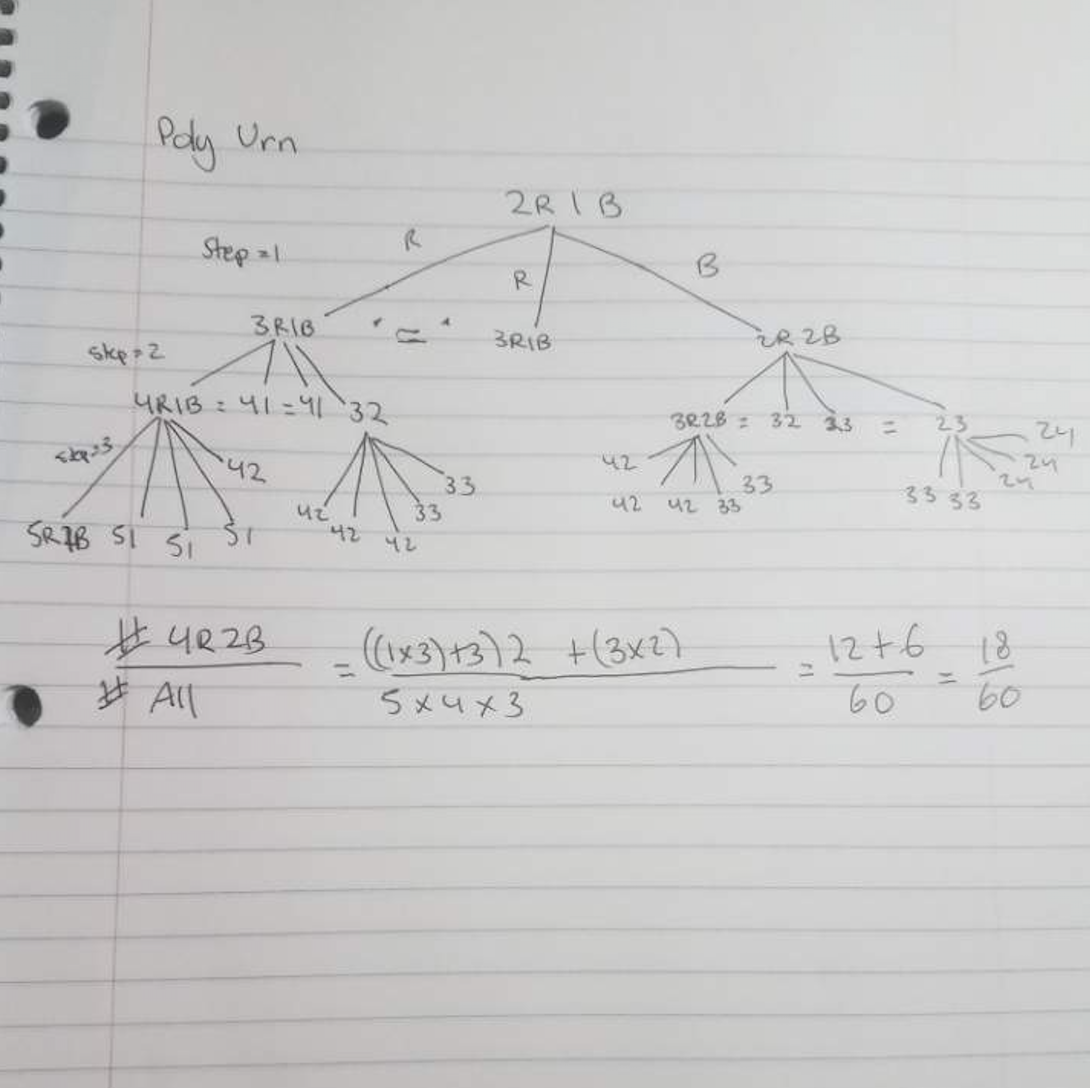
\includegraphics[scale=0.5]{polyurn.png}
\end{center}

\setcounter{section}{4}
\section{\sc\color{cit}Bayes' Rule}
\setcounter{subsection}{2}
\subsection{}
 \begin{enumerate}[(a)]
        \item 
        \begin{center}
        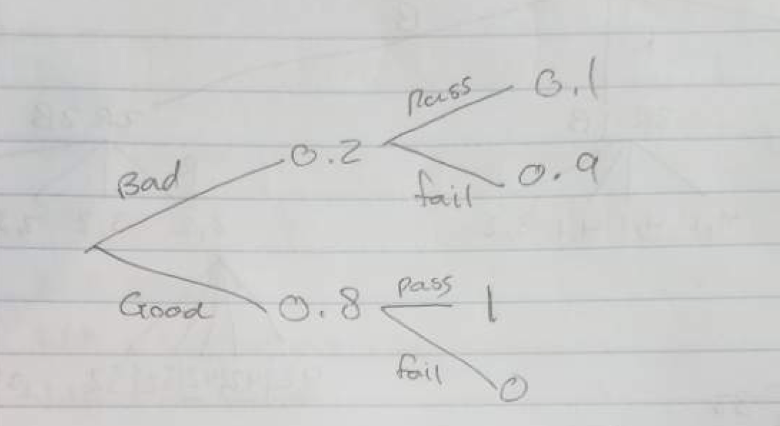
\includegraphics[scale=0.5]{chipgraph}
        \end{center}
        \begin{align*}
        P(bad) &= 0.2 \\
        P(pass | bad) &= 0.1 \\
        P(good | pass) & = ? \\
        &= \frac{\#(good pass)}{\#(pass)} \\        
        &= \frac{0.8}{(0.8*1) + (0.2*0.1)} \\
        &= \frac{0.8}{0.82} \\
        &= 0.97561 \\
        &= \mathbf{0.98}\\
        \end{align*}
        \item \begin{align*}
         P(bad) &= 0.2 \\
        P(pass | bad) &= 0.1 \\
        P(bad | pass) & = ? \\
        &= \frac{\#(bad pass)}{\#(pass)} \\        
        &= \frac{0.2*0.1}{(0.8*1) + (0.2*0.1)} \\
        &= \frac{0.02}{0.82} \\
        &= 0.02439 \\
        &= \mathbf{0.02}\\
        \end{align*}
    \end{enumerate}
    \setcounter{subsection}{6}
\subsection{}
 \begin{enumerate}[(a)]
 \item As shown in Example 1 we already have the probabilities for white...\ \\
 \begin{align*}
 P(\textnormal{Box 1} \mid \textnormal{white}) &= \frac{6}{23} \\
P(\textnormal{Box 2} \mid \textnormal{white}) &= \frac{8}{23} \\
P(\textnormal{Box 3} \mid \textnormal{white}) &= \frac{9}{23} \\
 \end{align*}
 Now using the same method we must find for black as well... \ \\
  \begin{align*}
 P(\textnormal{Box 1} \mid \textnormal{black}) &= \frac{6}{13} \\
P(\textnormal{Box 2} \mid \textnormal{black}) &= \frac{4}{13} \\
P(\textnormal{Box 3} \mid \textnormal{black}) &= \frac{3}{13} \\
 \end{align*}
 If we pick the highest posterior probability for both the chance of use being right over the long run is...\ \\
   \begin{align*}
  P(\textnormal{Box 1} \mid \textnormal{white}) * P(\textnormal{white})&+ P(\textnormal{Box 1} \mid \textnormal{black}) * P(\textnormal{black})  \\
\frac{9}{23} * \frac{23}{36} &+ \frac{6}{13} * \frac{13}{36} \\
&\mathbf{\frac{5}{12}}
 \end{align*}
\item This is problem 7c. Sorry for the confusion on ordering...\ \\
In this case the posterior probabilities will change ...
 \begin{align*}
 P(\textnormal{Box 1} \mid \textnormal{white}) &= \frac{9}{23} \\
P(\textnormal{Box 2} \mid \textnormal{white}) &= \frac{6}{23} \\
P(\textnormal{Box 3} \mid \textnormal{white}) &= \frac{27}{92} \\
 \end{align*}
 Now using the same method we must find for black as well... \ \\
  \begin{align*}
 P(\textnormal{Box 1} \mid \textnormal{black}) &= \frac{9}{13} \\
P(\textnormal{Box 2} \mid \textnormal{black}) &= \frac{3}{13} \\
P(\textnormal{Box 3} \mid \textnormal{black}) &= \frac{9}{52} \\
 \end{align*}
 If we pick the highest posterior probability for both the chance of use being right over the long run is...\ \\
   \begin{align*}
  P(\textnormal{Box 1} \mid \textnormal{white}) * P(\textnormal{white})&+ P(\textnormal{Box 1} \mid \textnormal{black}) * P(\textnormal{black})  \\
\frac{27}{92} * \frac{23}{36} &+ \frac{9}{13} * \frac{13}{36} \\
&\mathbf{\frac{7}{16}}
 \end{align*}
\end{enumerate}
\section{\sc\color{cit}Sequence of Events}
\setcounter{subsection}{5}
 \subsection{}
 \begin{enumerate}[(a)]
 \item First we can assume that the probability for $r = 1 $ and $r > 8 $ is $0 $.\ \\
 This is because in the case of $r = 1 $ there is no way of rolling the same number since you have not rolled at least twice.  \ \\
 The case for $r >8 $ is $0 $ as well since there are only six sides of a dice. There has to be a number that is repeated in this case since there isn't more (different options) the roll can output. . . \ \\
 All other options are computed below . . . 
  \begin{center}
 Table for all rolls... \\
 \ \\
 \begin{tabular}{ |c|c|c| }
 \hline
$r$ & computation & result \\
\hline
$1$ & $0 $ & $0$ \\
\hline
$2$ & $ (\frac{6}{6}) * (\frac{1}{6}) $ & $\frac{1}{6} $ \\
\hline
$3$ & $ (\frac{6}{6}) * (\frac{5}{6}) * (\frac{2}{6})$ & $\frac{5}{18} $ \\
\hline
$4$ & $ (\frac{6}{6}) * (\frac{5}{6}) * (\frac{4}{6}) * (\frac{3}{6})$ & $\frac{5}{18} $ \\
\hline
$5$ & $ (\frac{6}{6}) * (\frac{5}{6}) * (\frac{4}{6}) * (\frac{3}{6}) * (\frac{4}{6})$ & $\frac{5}{27} $ \\
\hline
$6$ & $ (\frac{6}{6}) * (\frac{5}{6}) * (\frac{4}{6}) * (\frac{3}{6}) * (\frac{2}{6}) * (\frac{5}{6})$ & $\frac{25}{324} $ \\
\hline
$7$ & $ (\frac{6}{6}) * (\frac{5}{6}) * (\frac{4}{6}) * (\frac{3}{6}) * (\frac{2}{6}) * (\frac{1}{6}) * (\frac{6}{6})$ & $\frac{5}{324} $ \\
\hline
$r \geq 8$ & $0 $ & $0 $ \\
\hline
 \end{tabular}
 \end{center}
 The logic behind this is for example take $r = 4 $. We can see that the first roll will not matter so there are $6 $ possible outcomes out of $6 $, which is represented by the first fraction. However, the next roll must be anything \textbf{except} that number chosen. This means the next probability is $\frac{5}{6} $. This process is done again to get $\frac{4}{6} $. However, for the last step we want to repeat one of the numbers already chosen. This means that we currently have three options to choose from, which gives us $\frac{3}{6} $. Multiply all these probabilities will give the result of $\frac{5}{18} $. 
 \item $p_1 + p_2 + ... + p_10 = \mathbf{1}$ \ \\
 This must be true because for a six-sided die there are only six options. The number must repeat for rolls of 7 above and it is zero for the middle layers of $r $. This equation covers all possibilities which is why it must equate to $1 $. 
 \item 
 \begin{align*}
 p_1 &+ p_2 + p_3 + p_4 + p_5 + p_6 + p_7 + p_8 +p_9 + p_10  = 1\\
 0 &+ \frac{1}{6} + \frac{5}{18} + \frac{5}{18} + \frac{5}{27} + \frac{25}{324} + \frac{5}{324} + 0 + 0 + 0 = 1 
 \end{align*}
 \end{enumerate}
 \setcounter{subsection}{7}
\subsection{}
 \begin{enumerate}[(a)]
 \item We can solve this problem by looking at this equation... 
 \begin{proof}
 \begin{align*}
 P(B_{12} \cap B_{23}) &= P( \textnormal{all have the same birthday}) \\
 \\
 \textnormal{Let's look at it seperatly...} \\
 \\
 P(B_{12}) &= \frac{365}{365} * \frac{1}{365} \\
 P(B_{23}) &= \frac{365}{365} * \frac{1}{365} \\
P( \textnormal{all have the same birthday}) &=\frac{365}{365} * \frac{1}{365} * \frac{1}{365} \\
\\
\textnormal{Based on the multiplication rule for independent events...} \\
\\
 P(B_{12} \cap B_{23}) &= P( \textnormal{all have the same birthday}) \\
  \frac{365}{365} * \frac{1}{365} *  \frac{365}{365} * \frac{1}{365} &=  \frac{365}{365} * \frac{1}{365} * \frac{1}{365} \\
  \frac{1}{365^2} &= \frac{1}{365^2} 
 \end{align*}
 Because this equality holds for independent events we can say that they are independent. \\
 \end{proof}
 \item \begin{proof}
 This is not independent. The $B_{12} $ and $B_{23} $ implies that $B_{13} $ based on the definition. Also using the same logic as above the equation will be ... \\
 $ \frac{1}{365^2} = \frac{1}{365^3} $ which is not true.\ \\
 \end{proof}
 \end{enumerate}
\setcounter{chapter}{2}
\setcounter{section}{0}
\section{\sc\color{cit}Distributions}
\setcounter{subsection}{6}
\subsection{}
 \begin{enumerate}[(a)]
 \item We can do this with Binomial Distribution. However, we are missing some information. We have $n$, $k$, but we must calculate $p$... 
   \begin{center}
 Ways to win... \\
 \ \\
 \begin{tabular}{ |c|c|c| }
 \hline
Opponent & Me & \#ways \\
\hline
$1$ & $2, 3, 4, 5, 6 $ & $5$ \\
\hline
$2$ & $ 3, 4, 5, 6 $ & $4$ \\
\hline
$3$ & $ 4, 5, 6 $ & $3$ \\
\hline
$4$ & $ 5, 6$ & $2$ \\
\hline
$5$ & $ 6$ & $1 $ \\
\hline
$6 $ & N/A & $0 $ \\
\hline
 \end{tabular}
\begin{align*}
\textnormal{Total number of ways to win} &= 15 \\
\textnormal{Total combinations} &= 36 \\
P(winning) = p &= \frac{5}{12}
\end{align*}
 \end{center}
 Let us apply Binomial Distribution ... \\
 \begin{align*}
 P(k \textnormal{ success in } n \textnormal{ trials}) &= \binom{n}{k}p^kq^{n-k}  \\
  P(4 \textnormal{ success in } 5 \textnormal{ trials}) &= \binom{5}{4}\bigg(\frac{5}{12}\bigg)^4\bigg(\frac{7}{12}\bigg)^{1}  \\
 \end{align*}
 However we must also look at $5 $ since the question was at least $4 $...
  \begin{align*}
 P(k \textnormal{ success in } n \textnormal{ trials}) &= \binom{n}{k}p^kq^{n-k}  \\
  P(4 \textnormal{ success in } 5 \textnormal{ trials}) &= \binom{5}{5}\bigg(\frac{5}{12}\bigg)^5\bigg(\frac{7}{12}\bigg)^{0}  \\
 \end{align*}
 The two Probabilities added together is $0.10047$ \\
 The probability of winning at least $4 $ times is $\mathbf{0.10047}$
\end{enumerate}
\setcounter{subsection}{9}
\subsection{}
 \begin{enumerate}[(a)]
 \item \begin{align*}
 P(k -1 \textnormal{ heads } | k-1 \textnormal{ or } k \textnormal{ heads}) \\
 &= \frac{P(k-1 \textnormal{ heads }) \cap P(k-1 \textnormal{ or } k \textnormal{ heads})}{P(k-1 \textnormal{ or } k \textnormal{ heads})}\\
 &= \textnormal{ the numerator will equate to just } P(k-1 \textnormal{ heads})\\ &\textnormal{ this is because the definition of intersection} \\
 &= \frac{P(k-1 \textnormal{ heads })}{P(k-1 \textnormal{ or } k \textnormal{ heads})}\\
 &= \textnormal{The denominator will equate to the addition of the two or cases} \\
&= \frac{P(k-1 \textnormal{ heads })}{P(k-1 \textnormal{ heads }) + P(k \textnormal{ heads } )} \\
&= \frac{\binom{n}{k-1}}{\binom{n}{k-1} + \binom{n}{k}} \\
&= \frac{\frac{n!}{(k-1)!(n-k-1)!}}{\frac{n!}{(k-1)!(n-k-1)!} * \frac{n!}{(k)!(n-k)!}} \\
&= \frac{k}{k+n-k+1} \\
&= \frac{k}{n+1} \\
 \end{align*}
 \item This is $1 - $ above ... \ \\
 \begin{align*}
 1 - \frac{k}{n+1} \\
 \frac{n+1-k}{n+1} \\
 \end{align*}
 \end{enumerate}
 \setcounter{section}{4}
\section{\sc\color{cit}Random Sampling}
\setcounter{subsection}{1}
\subsection{}
 \begin{enumerate}[(a)]
\item \begin{align*}
P(\textnormal{ First is red } ) &= \frac{26}{52} \\
P(\textnormal{ Second is Black } ) &= \frac{26}{51} \\
P(\textnormal{ Third is Black } ) &= \frac{25}{50} \\
P(\textnormal{  First card is red and the second two black } ) &= \frac{13}{102} \\
&= \mathbf{0.12745}
\end{align*}
\item For this problem we can use the formula given on page 125 for sampling without replacement!
\begin{align*}
P(1 \textnormal{ red and } 2 \textnormal{ black}) &= \frac{\binom{26}{1} * \binom{26}{2}}{\binom{52}{3}} \\
&=\frac{\frac{26*26*25}{2}}{\frac{52*51*50}{3*2}} \\
&=\frac{39}{102} \\
&= \frac{13}{34} \\
&= \mathbf{0.38235}
\end{align*}
\item We can use the above procedure to find the Probability when there is 1 red, 2 red, or 3 red.
\begin{align*}
P(1 \textnormal{ red and } 2 \textnormal{ black}) &= \frac{\binom{26}{1} * \binom{26}{2}}{\binom{52}{3}} \\
&=\frac{\frac{26*26*25}{2}}{\frac{52*51*50}{3*2}} \\
&=\frac{39}{102} \\
&= \frac{13}{34} \\
&= \mathbf{0.38235} \\
\\
P(2 \textnormal{ red and } 1 \textnormal{ black}) &= \frac{\binom{26}{2} * \binom{26}{1}}{\binom{52}{3}} \\
&=\frac{\frac{26*26*25}{2}}{\frac{52*51*50}{3*2}} \\
&=\frac{39}{102} \\
&= \frac{13}{34} \\
&= \mathbf{0.38235} \\
\\
\textnormal{ the next 3 red is just ... } \\
P(3 \textnormal{ red and } 0 \textnormal{ black}) &= \frac{26}{52} * \frac{25}{51} * \frac{24}{50} \\
&= \frac{2}{17} \\
& = \mathbf{0.11764}
\end{align*}
Summing all those probabilities together you get $\mathbf{0.88235} $
\end{enumerate}
\setcounter{subsection}{6}
\subsection{}
 \begin{enumerate}[(a)]
 \item This is the probability of choosing consecutive 4 black balls.
\ \\
$\frac{50}{80} * \frac{49}{79} * \frac{48}{78} *\frac{47}{77} = \mathbf{0.1456} $
\item This the probability of choosing exactly three black balls is ... \ \\
$\frac{50}{80} * \frac{49}{79} * \frac{48}{78} * \frac{30}{77} * 4 = \mathbf{0.3717} $
\item The probability that the first red ball appears on the last draw is ... 
\ \\
$\frac{50}{80} * \frac{49}{79} * \frac{48}{78} * \frac{30}{77} =\mathbf{0.0929} $
 \end{enumerate}
\end{document}
